\documentclass[a4paper,10pt]{article}
\usepackage[utf8]{inputenc}
\usepackage[T1]{fontenc}
\usepackage[french]{babel}
\usepackage{graphicx}
\usepackage[font=small,labelfont=bf]{caption}
\usepackage{amsmath}
\usepackage{stackengine}

\newcommand\tabA[1][0.5cm]{\hspace*{#1}}
\newcommand\tabB[1][1.5cm]{\hspace*{#1}}
\newcommand\tabC[1][2cm]{\hspace*{#1}}
\setlength{\parindent}{0cm}
\setlength{\parskip}{1ex plus 0.5ex minus 0.2ex}
\newcommand{\hsp}{\hspace{20pt}}
\newcommand{\HRule}{\rule{\linewidth}{0.5mm}}


% Title Page
\begin{document}
\begin{titlepage}
  \begin{sffamily}
  \begin{center}

    % Upper part of the page. The '~' is needed because \\
    % only works if a paragraph has started.
    
\includegraphics{./image/ua_v_couleur.jpg}
    
    \textsc{ UNIVERSIT\'{E} D'ANGERS \\ UFR INFORMATIQUE}\\[0.5cm]
    \textsc{ \\ Rapport de stage \\ Master 1 2016-2017 }\\[1.5cm]
    
    
\includegraphics{./image/logo-generique-SD.png}
    
    \textsc{UMR INSERM 1232 \\-Equipe Immunité Innée et Immunothérapie}\\[1cm]
     
    % Title
    \HRule \\[0.4cm]
    { \huge \bfseries ANALYSE TRANSCRIPTOMIQUE\\[0.4cm] }

    \HRule \\[2cm]

    % Author and supervisor
    \begin{minipage}{0.4\textwidth}
      \begin{flushleft} \large
        \large Présenté par : \\\textsc{RASOLONIAINA Marlino}
      \end{flushleft}
    \end{minipage}
    \begin{minipage}{0.4\textwidth}
      \begin{flushright} \large
        \emph{Tuteur :} M. Le \textsc{Tuteur}\\
        \emph{Chef d'équipe : } M. Chef \textsc{D’Équipe}
      \end{flushright}
    \end{minipage}

    \vfill

    % Bottom of the page
    {\large 12 Avril 2017 — 20 Juin 2017}

  \end{center}
  \end{sffamily}
\end{titlepage}
\newpage
\tableofcontents
\newpage
\section{INTRODUCTION :}
\section{ACQUISITION DES DONN\'{E}ES :}
\subsection{Les puces à ADN :}
  Une puce à ADN est constituée d'un support physique (le plus
  souvent une lame de verre) sur lequel sont déposées des molécules
  d'ADN correspondant à de petits fragments du génome (jusqu'à 40 000
  dépôts différents par puce). On recouvre la puce
  de la solution contenant la population d'ARN à étudier. Les ARN
  s'hybrident sur les fragments d'ADN complémentaires. La quantité d'ARN
  fixée reflète la concentration de cet ARN dans la solution.
  \newline
 Pour des raisons pratiques, on utilise des ADNc plutôt que directement
  les ARN. Les ADNc sont marqués par un nucléotide radioactif ou
  un fluorochrome. Il est possible d'étudier simultanément plusieurs
  populations d'ADNc sur une même puce en utilisant des fluorochromes différents.
  La meilleure façon d'utiliser cette possibilité est de marquer
  l'ADN génomique avec un fluorochrome, toujours le même. On
  obtient ainsi une référence stable au cours des années
  qui permet de mettre toutes les puces à la même échelle,
  quelle que soit leur origine. 
  \newline
  Un scanner mesure l'intensité du signal émis par l'ADNc hybridé au niveau de chaque dépôt. Parmi les valeurs que proposent les
  logiciels pour cette intensité, la plus fiable est la médiane de l'intensité des pixels car elle est moins sensible aux défauts de
  l'image (pixels sur-brillants par exemple). 
  \newline
  Les puces comportent généralement plusieurs dépôts identiques pour chaque gène. Cela simplifie le travail lorsqu'il faut
  repérer les aberrations dans la lecture des intensités puisqu'il suffit d'examiner les cas où les valeurs diffèrent beaucoup d'un
  dépôt à l'autre. Il s'agit le plus souvent d'un défaut physique sur la puce et il est facile d'éliminer la valeur aberrante.
  Dans le doute, on conserve la médiane des différentes mesures. 
  \newline
  Plusieurs  types  de  puces  à  ADN  
existent selon le support, la nature des fragments fixés à la surface, le mode de fabrication, la 
densité, le mode de marquage des cibles et les méthodes d’hybridation.
\begin{center}
 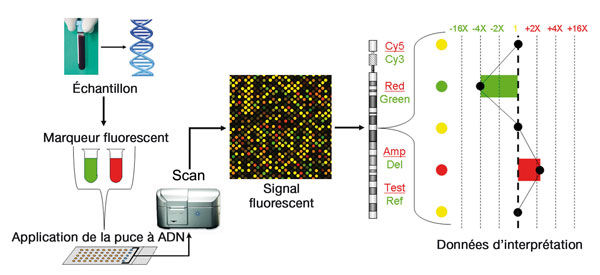
\includegraphics[scale=0.5]{./image/principe.jpg}
 % Etapes_d'une_expérience_de_biopuces.png: 0x0 pixel, 300dpi, 0.00x0.00 cm, bb=
 \captionof{figure}{Principe général d'utilisation des puces ADN }
\end{center}

\subsection{La technologie Illumina :}
Illumina, Inc. est une société américaine qui fabrique et commercialise des systèmes intégrés pour l'analyse de la variation génétique et la fonction biologique 
notamment des gammes de produits et services qui servent les marchés du séquençage, génotypage et expression génétique.
\newline
Une de ces récentes fabrications, la puce ``BeadArray technologie''.
\begin{center}
 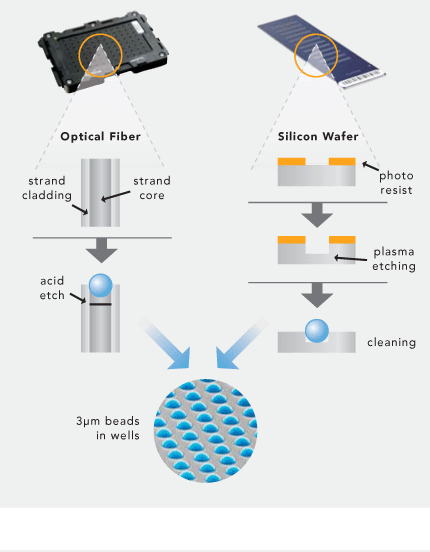
\includegraphics[scale=0.5]{./image/beadarray.png}
 % beadarray_multi_sample_array_formats_lg.gif: 0x0 pixel, 300dpi, 0.00x0.00 cm, bb=
 \captionof{figure}{Illumina BeadArray Technologie }
\end{center}
Dans l’analyse des expressions des gènes, Illumina utilise deux approches différentes : l’hybridation directe(Direct Hybridization assay) et le DASL (cDNA-mediated Annealing Selection Extension and Ligation).
L’expérience est faite avec la première approche qui consiste à utiliser un simple brin de la séquence d’ADN par spot. Cette séquence monocaténaire est censée s’hybrider avec la séquence cible étiquetée dans l’échantillon. 
La quantité du signal fluorescente produit détermine la quantité de l’ARN cible dans l’échantillon.
\begin{center}
 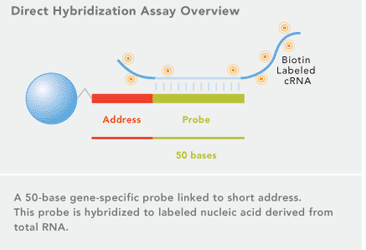
\includegraphics[scale=0.5]{./image/Direct_Hyb.png}
 % direct_hybridization_assay_workflow_lg.png: 0x0 pixel, 300dpi, 0.00x0.00 cm, bb=
 \captionof{figure}{An Illumina Direct Hybridization probe }
\end{center}
\begin{center}
 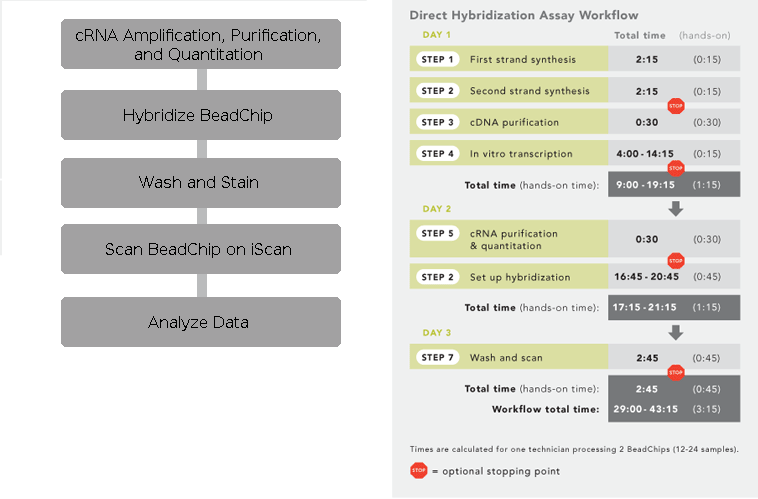
\includegraphics[scale=0.5]{./image/direct_hybridization_assay_workflow.png}
 % direct_hybridization_assay_workflow.png: 0x0 pixel, 300dpi, 0.00x0.00 cm, bb=
 \captionof{figure}{ Direct Hybridization assay workflow}
\end{center}

\subsection{ Plan expérimental :}
\begin{center}
 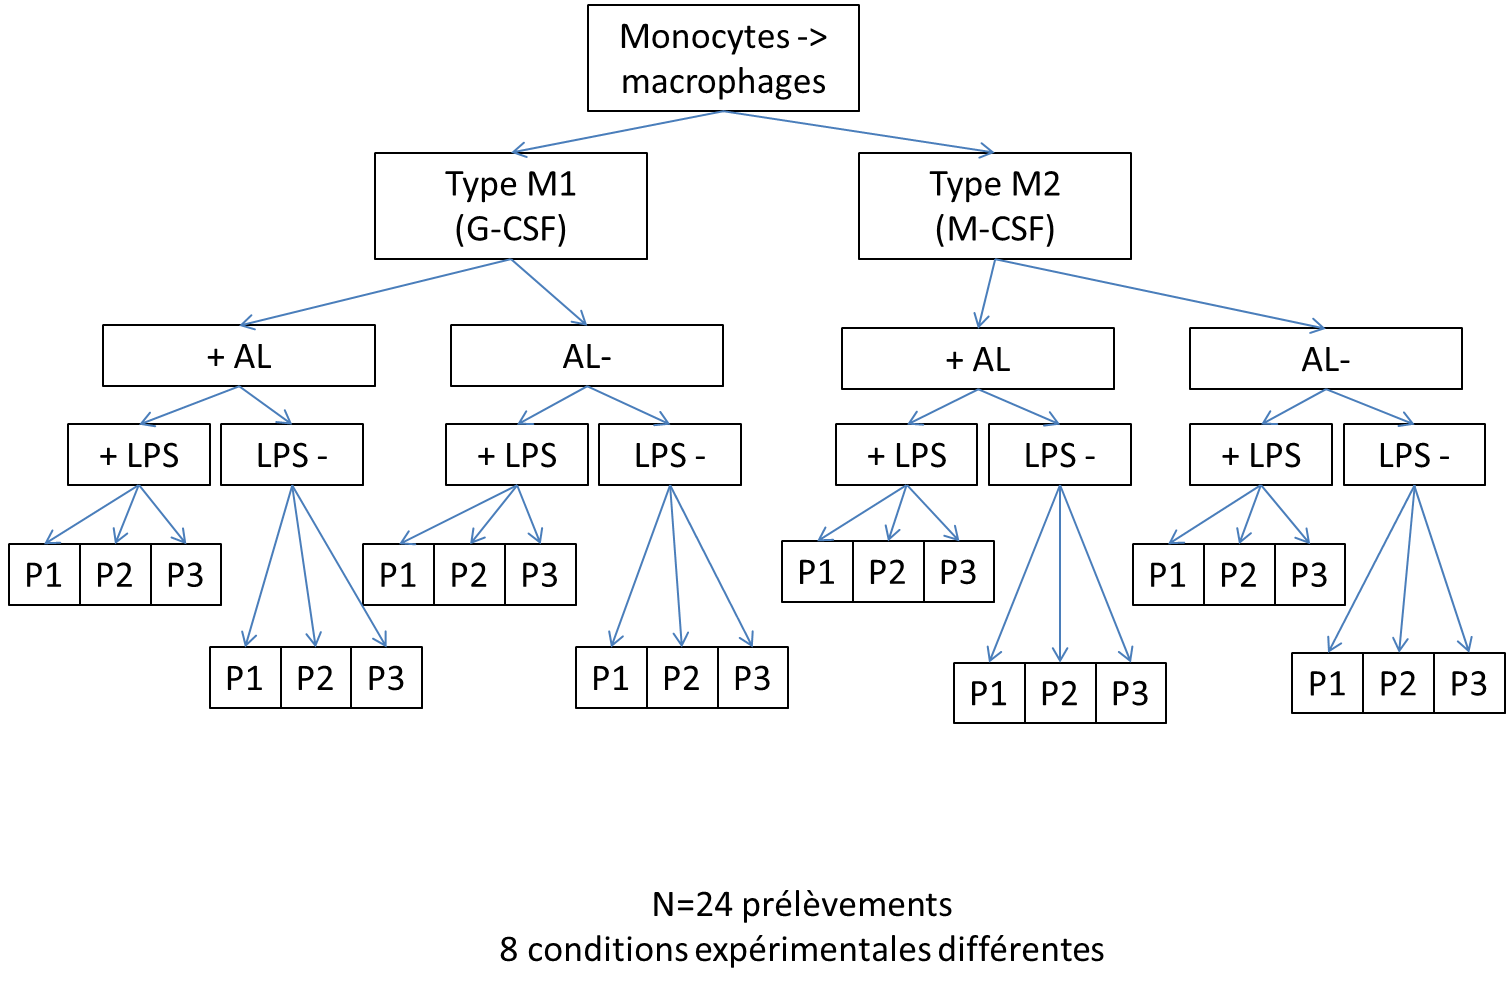
\includegraphics[scale=0.5]{./image/plan.png}
 % plan.png: 0x0 pixel, 300dpi, 0.00x0.00 cm, bb=
 \captionof{figure}{Plan éxpérimental }
\end{center}
L’expérience a été faite avec la puce ADN  Illumina HumanHT-12 v4.0 BeadChip 12x1 avec 48210 sondes pour chaque prélèvement.
887 de ses sondes sont classés comme des sondes de contrôles.
On se trouve donc avec 47323 individus sur 24 variables. 
Ce qui nous donne une matrice de données de dimmension :
\def\tmp{
  \begin{pmatrix}
  a_{11} & \cdots & a_{1m} \\

   \vdots & \ddots &\vdots \\

   a_{n1} & \cdots & a_{nm} 
 \end{pmatrix}
}
\[
\stackMath\def\stackalignment{r}
  \stackon
    {\mathrm{47323~rows}\left\{\tmp\right.}
    {\overbrace{\phantom{\smash{\tmp\mkern -36mu}}}^{\mathrm{\textstyle 24~columns}}\mkern 20mu}
\]

\subsection{Les sources de variations et les défis sur l'utilisation des puces ADN :}

La littérature nous raconte que si on effectue à plusieurs reprises une même expérience, on peut se heurter à des valeurs d’expérience légèrement différentes à chaque exécution.
Il est de ce fait très intéressant de voir de plus près les grandes étapes et les effets des processus biologiques qui sont derrières ces sources de quantité de variabilité dans l’étude des expressions génomique avec les puces ADN.
De ce point de vue, ces variations sont considérées comme des bruits dans la phase d’analyse des expressions.\\
Est-ce que la variation d’un gène particulier est due au bruit de fond de la puce ou c’est réellement une différence entre les différentes expériences testées ? C’est là le vrai challenge. 
Si on prend un gène spécifique, combien de quantité de sa valeur représente la mesure de la variance due à la régulation des gènes et due à la quantité de bruit ?
Néanmoins, une grande partie de la variabilité induite par la puce elle-même  peut être déterminée à l'aide des techniques 
de réplications ou d’autres techniques de séparations des bruits (Exemples : conception d’expérience statistique, normalisation des données). 
\begin{table}[!ht]
\begin{tabular}{|l|p{6cm}|}
\hline
 Facteur & Commentaires\\
\hline
Préparation des mRNA et la transcription &  Tissus, les kits et les procedures variantes \\
\hline 
Transcription & Les variations inhérentes dans la réaction, le type de l'enzymes utilisé  \\
\hline 
L'étiquetage (Labeling) & Depend du type,des procédures et l'âge de l'étiquette  \\
\hline
Amplification (PCR) & Il est difficille de quantifier le rendement du PCR\\
\hline
Variations géométriques des broches & différentes surfaces et propriétés dues à des erreurs aléatoires de production \\
\hline
Volume de l'échantillon & fluctue stochastiquement même pour la même broche (pin)  \\
\hline
Fixation de l'échantillon & La fraction de l'ADNc cible (une gouttelette) qui est chimiquement liée à la surface de la diapositive n'est pas prise en compte \\
\hline
 Paramètre d'hybridation&  influencé par plusieurs facteurs comme la temperature,le temps,le buffering \\
\hline
 Hybridation non-spécifique& un ADNc s'hybride avec une sequence qui n'est pas exactement son complémentaire \\
\hline
Réglages de gain & déplace la répartition des intensités de pixels \\
\hline
Limitation de la plage dynamique & Variabilité de la saturation au bas de gamme ou au haut de gamme \\
\hline
Alignement d'image & Les images d'un même BeadArray à diverses longueurs d'onde correspondant à des canaux différents ne sont pas alignées; différents pixels sont considérés pour le même emplacement \\
\hline
 Placement de la grille& le centre du spot n’est pas bien localisé  \\
\hline
 Bruit de fond non-spécifique& Élévation erronée de la moyenne de l'intensité du bruit de fond \\
\hline
Forme de spot & L'intensité des spots irréguliers sont difficille à segmenter en bruit de fond \\
\hline
 Segmentation& Des contaminants lumineux peuvent ressembler comme un signal(ex: poussière) \\
\hline
 Quantification de spot& la moyenne des pixels, la médiane,... \\
\hline
\end{tabular}
\caption{Sources of fluctuations in a typical cDNA microarray experiment}
\label{Sources de variation}
\end{table}
\section{DESCRIPTION DES DONN\'{E}ES :}
\subsection{ Décryptage et lecture :}
Après avoir scanné la puce, le scanner iScan d’Illumina exporte et produit des fichiers de sortie selon les paramètres définis.
Les fichiers qui contiennent les intensités des spots (.idat) sont encryptés et d’autres fichiers sont fournis à titre indicatif et de mesure pour l’analyse.\\
\begin{table}[!ht]
\begin{tabular}{|l|p{9cm}|}
\hline
File  & Description \\
\hline
 (Serial Number).txt & un fichier qui stocke la positions et l'identité de chaque spots, qui contient quelques informations sur les paramètres du scanner\\
\hline
Metrics.txt &  un pour chaque BeadChip  et contient des informations récapitulatives sur l'intensité des signals,
la quantité de saturation, la mise au point et l'enregistrement sur l'image (s) de chaque section \\
\hline 
Effective.cfg & fichier de configuration des paramètres du scanner\\
\hline
(Serial Number).sdf & fichier de description des échantillons d'Illumina utilisé pour déterminer les propriétes (positions)
physique d'une section et savoir les sections liées sur chaque échantillons\\
\hline
*.idat & contiennent la moyenne des intensités du signal de chaque spots \\
\hline
\end{tabular}
\caption{Description des fichiers de sortie}
\label{Fichiers_Sorties}
\end{table}
\newline
Pour la lecture  des fichiers .idat, l’utilisation d’un fichier manifeste qui contient l’ensemble de tout les informations nécessaires concernant la puce est indispensable pour le décryptage : le nom et l’identifiant  des gènes ( Probe\_id, Array\_Address\_Id, Symbol, Barcode), le statut d’un spot (regular, negative, biotin,...)
Dans la suite logique des choses, Illumina fourni un logiciel payant (GenomeStudio Software)  qui aide sur le traitement et l'analyse des puces ADN (Genotyping Module, Gene Expression Module, Methylation Module).
\subsection{ Données brutes via Bioconductor :}
Bioconductor est un projet de développement et un ensemble de package (1380 packages en 2017)  gratuit et open source dans l’analyse et la compréhension des données génomiques basé principalement en langage de programmation statistique R.
Limma est un des packages dans Bioconductor pour l’analyse des expressions génomique des puces  ADN. La function read.idat de package Limma permet de lire les fichiers idat d’Illumina BeadArray en fournissant en paramètre le fichier manifeste .bgx correspondant à la plateforme d’expression de gène à étudier.
On obtient après un objet limma de type EListRaw  qui contient les objets suivants:
\begin{table}[!ht]
\begin{tabular}{|l|p{9cm}|}
\hline
 \emph{E} & matrice des intensité brutes\\
\hline
\emph{other\$NumBeads }   &  matrice de mêmes dimensions que E donnant les nombre de spots (bead) utilisées pour chaque valeur d'intensité. \\
\hline 
\emph{other\$STDEV} & matrice de mêmes dimensions que E donnant un écart type au niveau des spots ou une erreur standard pour chaque valeur d'intensité.\\
\hline
\emph{genes} & un data.frame des annotations des sondes qui contient des informations extraites du fichier manifeste relatif au type de puce utilisé : Probe\_Id, Array\_Address\_Id, Status
\\
\hline
\end{tabular}
\caption{Contenu de l'objet EListRaw retourné par la fonction read.idat() de limma}
\label{EListRaw}
\end{table}
\subsection{ Contrôle et qualité :}

\section{PR\'{E}TRAITEMENT DES DONN\'{E}ES :}
\subsection{Transformation :}
\subsection{Normalisation :}
\subsection{Filtrage :}

\section{ANALYSE DES DONN\'{E}ES DE TRANSCRIPTOME :}
\subsection{Gènes différentiellement exprimés :}
\subsection{Gènes co-exprimés :}

\section{INTERP\'{E}TATION :}
Caractérisation d’un ensemble de gènes
\begin{abstract}
\end{abstract}
\end{document}          
